% Created 2016-01-27 Wed 09:13
\documentclass[bigger]{beamer}
\usepackage[utf8]{inputenc}
\usepackage[T1]{fontenc}
\usepackage{fixltx2e}
\usepackage{graphicx}
\usepackage{longtable}
\usepackage{float}
\usepackage{wrapfig}
\usepackage{rotating}
\usepackage[normalem]{ulem}
\usepackage{amsmath}
\usepackage{textcomp}
\usepackage{marvosym}
\usepackage{wasysym}
\usepackage{amssymb}
\usepackage{hyperref}
\usepackage{multicol}
\usepackage{caption}
\tolerance=1000
\usetheme{default}
\author{Nooreen S Dabbish and Kaijun Wang}
\date{Feb 1, 2016}
\title{Structure of and Inquiries about Healthy Connectivity Matrix Data}
\hypersetup{
  pdfkeywords={},
  pdfsubject={STAT 9190 presentation on data structure and summary with plots and identification of scientifically interesting questions.},
  pdfcreator={Emacs 24.4.1 (Org mode 8.2.10)}}
\begin{document}

\maketitle
\begin{frame}{Outline}
\tableofcontents
\end{frame}


\section{Data Structure}
\label{sec-1}
\subsection{Introduction to connectivity matrix data}
\label{sec-1-1}
\begin{frame}[label=sec-1-1-1]{Basics}
How it is organized. What types; what measurements are selected?
\end{frame}
\begin{frame}[label=sec-1-1-2]{Connectivity Matrices}
\begin{itemize}
\item symmetric/undirected n x n matrix
\item n x 3 list of Montreal Neurological Institute (MNI) coodinate spaces for each node
\item n x 1 lists of node names and abbreviations

\item\relax [data types] fMRI, Diffusion Tensor Images (DTI), Diffusion Spectrum Images (DSI), structural MRI, EEG, MEG
\end{itemize}
\end{frame}


\subsection{UMCD: USC Multimodal Connectivity Database}
\label{sec-1-2}
\url{http://umcd.humancommectomeproject.org}

\begin{frame}[label=sec-1-2-1]{Description in (Brown 2016)}
\begin{itemize}
\item central repository for connectivity matrices
\item click-of-the-mouse analyses
\item (as of 1/17/16) 2254 brain networks (CMs), 21 studies
\item all ages fetus to 89 yo.
\item healthy, ADHD, autism, OCD, APOE-4 carrier status (risk for AD)
\end{itemize}
\end{frame}

\subsection{Our particular dataset}
\label{sec-1-3}
\begin{frame}[label=sec-1-3-1]{Bejing Zang}
The dataset to be used: R-fMRI BOLD data from 148 subjects (74 female and 74
male; matched by age (21 years old) recruited as part of
larger studies conducted in Beijing China.

See the MATERIALS AND METHODOLOGY, Resting State Data of  
\url{http://www.ncbi.nlm.nih.gov/pmc/articles/PMC3271304/pdf/TONIJ-6-1.pdf}
\end{frame}


\section{Summary Plots and Numbers:}
\label{sec-2}
\subsection{Overview}
\label{sec-2-1}
\begin{frame}[label=sec-2-1-1]{Overview}
number of samples/variables/..histogram plot of some measurement 
to give a ``feel'' for the data. List of interesting modeling questions 
and why they are scientifically interesting?        
\end{frame}

\subsection{Correlation Plots}
\begin{frame}
\label{sec-2-2}
\begin{multicols}{2}
	\begin{center}
	Before Thresholding
    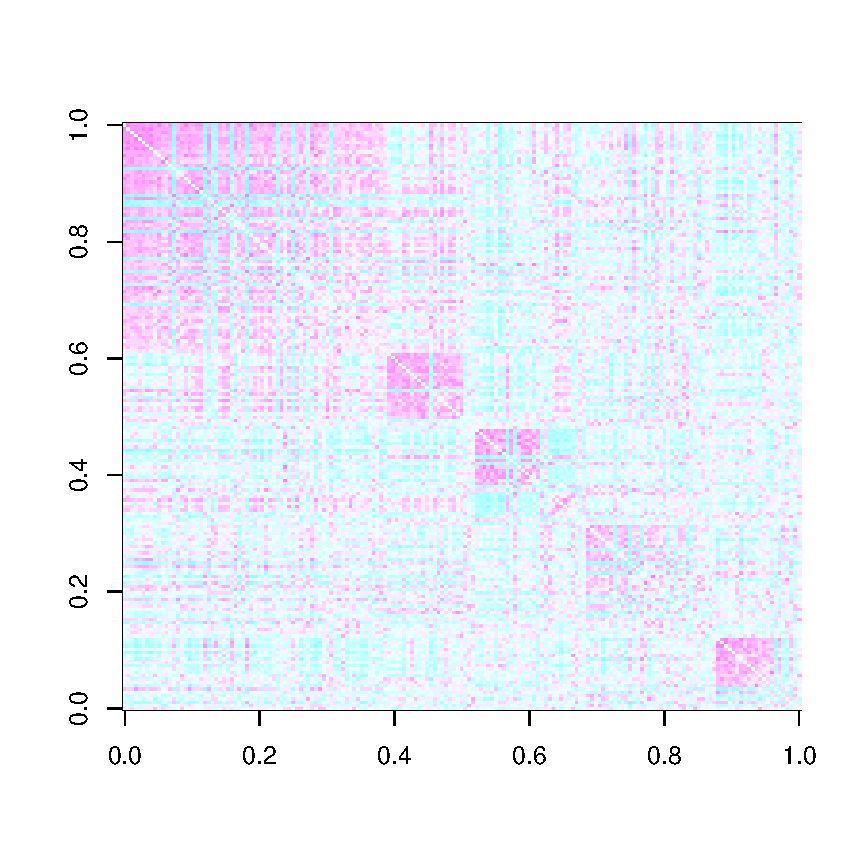
\includegraphics[height=2.3in,width=2.3in]{correlationplot_data37.pdf}
    \end{center}
    \begin{center}
    After thresholding (with 0.5)
     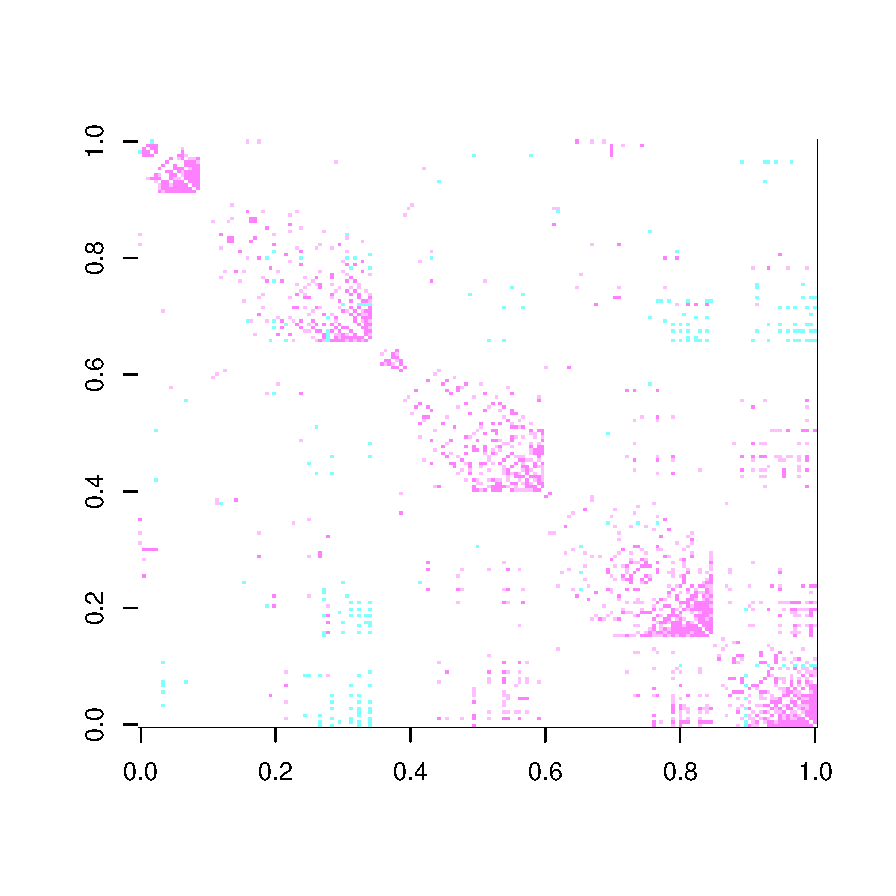
\includegraphics[height=2.3in,width=2.3in]{sparse_corr.eps}
    		%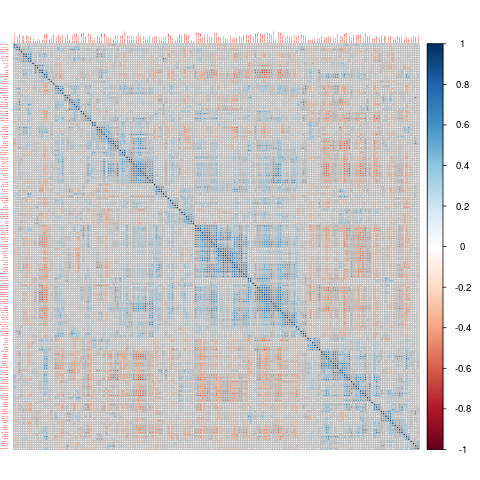
\includegraphics[height=2.3in,width=2.3in]{corrplot.png}
    \end{center}
\end{multicols}
\end{frame}

\subsection{qgraph, spring layout}
\label{sec-2-3}
\begin{frame}
\begin{multicols}{2}
\begin{center}
	Before Thresholding\\
	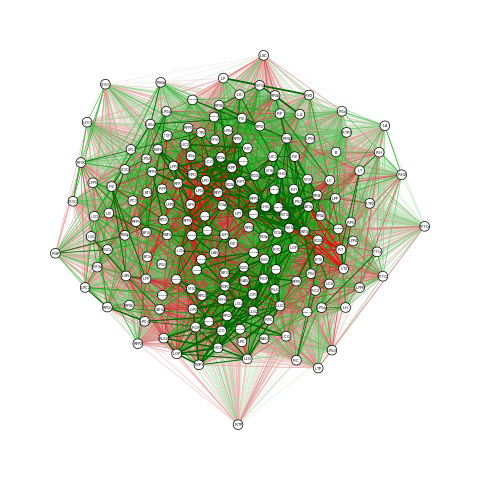
\includegraphics[height=2.2in,width=2.2in]{qgraph.png}
\end{center}
\begin{center}
	After Thresholding\\
	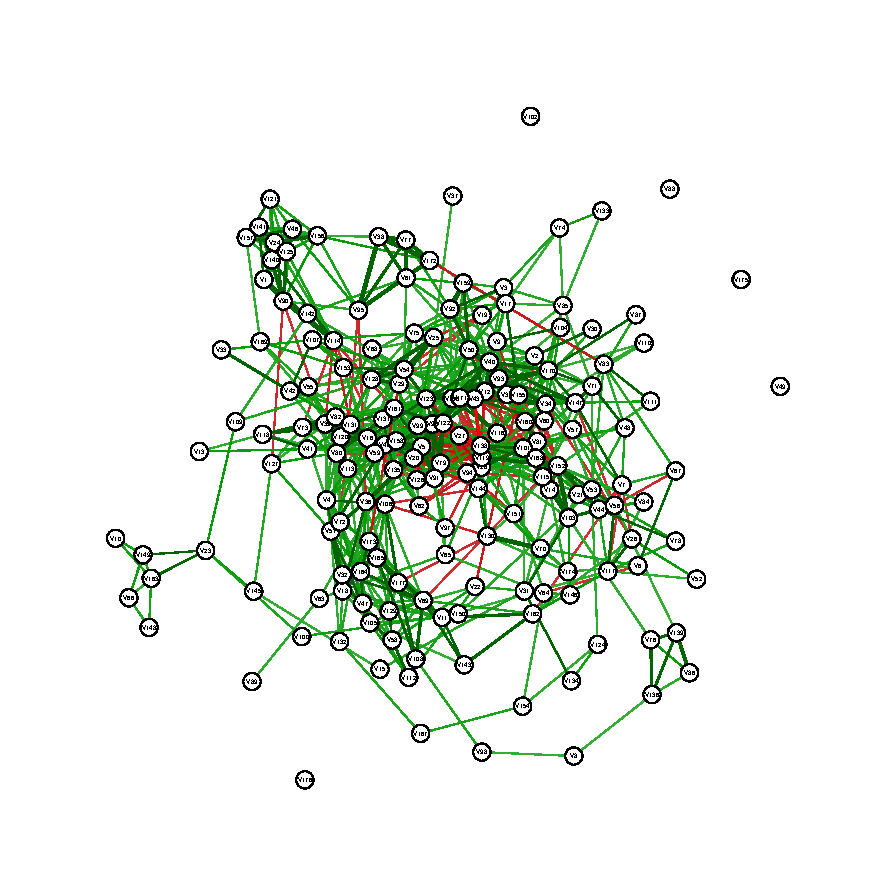
\includegraphics[height=2.2in,width=2.2in]{qplotpt5.eps}
\end{center}
\end{multicols}
% Emacs 24.4.1 (Org mode 8.2.10)
\end{frame}

\subsection{Degree Distribution}
\label{sec-2-4}
\begin{frame}
\begin{center}
	\includegraphics[width=4in,height=2.3in]{distpt5.eps}
\end{center}
	% Emacs 24.4.1 (Org mode 8.2.10)
\end{frame}

\section{Literature Research}
\subsection{Raw data preparation and processing}
\begin{frame}[label=sec-3-1]{Literatures: On fMRI Data}
\label{sec-3-1}
\begin{itemize}
\item Network Centrality in the Human Functional Connectome
Xi-Nian Zuo, et al.
(2011)\\

\item Toward reliable characterization of functional homogeneity in the human brain:
Preprocessing, scan duration, imaging resolution and computational space 
Xi-Nian Zuo, et al.
(2013)\\

\item Fully exploratory network independent component analysis of the 1000 functional connectomes database
Klaudius Kalcher, et al.(2013)
\end{itemize}
\end{frame}

\subsection{Classification:}
\begin{frame}[label=sec-3-2-1]{Literatures: Classification Problems}
\label{sec-3-2-1}
\begin{itemize}



\item Combining Graph and Machine Learning Methods to Analyze Differences
in Functional Connectivity Across Sex (2012)
Casanova R., et al.

Response: Gender

Random forest and Lasso

\item The Kernel Two-Sample Test for Brain Networks,
Emanuele Olivetti et al. (2015)

Response: Gender

Classification based method vs Kernel Two-sample
\end{itemize}
\end{frame}

\subsection{Classification2}
\begin{frame}[label=sec-3-2-2]{Literatures: Classification Problems}
\label{sec-3-2-2}
\begin{itemize}
\item Distinct neural signatures detected for ADHD subtypes after controlling for micro-movements in resting state functional connectivity MRI data
Damien A. Fair, et al. (2013)

Response: ADHD

\item The Autism Brain Imaging Data Exchange: Towards Large-Scale Evaluation of the Intrinsic Brain Architecture in Autism 
Di Martino, et al.(2014)

Response: Autism Spectrum Disorders

Intrinsic Functional Connectivity Analyses between Autism and Control Group
\end{itemize}
\end{frame}

\section{Possible Topics}
\begin{frame}[label=sec-4-1-1]{Possible Topics}
	\label{sec-4-1-1}
\begin{itemize}
	\item Classification according to the connectivity matrices, given exogenous data.
	\item Signal Path Clustering, normal pattern in brain activities
	\item Evaluate different classification methods on this data (e.g. random forest and lasso in [Cassanova 2012])
\end{itemize}
\end{frame}


\section{Methods}
\subsection{Graph Kernel}
\begin{frame}[label=sec-5-1-1]{Graph Kernel}
	\label{sec-5-1-1}
\begin{center}
	Graph pairs $G_i,G_j$ $\rightarrow$ Kernel $k_{ij}=\kappa(G_i, G_j)$ $\rightarrow$ Classifier 
\end{center}
\end{frame}

\subsection{Two-sample Test}
\begin{frame}[label=sec-5-1-2]{KTST}
	\label{sec-5-1-2}
Functional connectomes, 148 graphs, 74 from group A and 74 from group B

Kernel matrix: 148-by-148, of pairwise kernels
\begin{center}
	\begin{tabular}{c|c c c c c c c c}
		graphs & $A_1$ & $A_2$ & $\cdots$ & $A_m$& $B_1$ & $B_2$ & $\cdots$ & $B_n$ \\
		\hline
		$A_1$ & $k_{A1,A1}$ & $k_{A1,A2}$ & $\cdots$ & & $k_{A1,B1}$ & $\cdots$ & &\\
		$A_2$ & $k_{A2,A1}$& & & & & & &\\
		$\vdots$ &$\vdots$ & &$\ddots$ & & & & &\\
		$A_m$ & $k_{Am,A1}$ & $\cdots$ & & & & & &\\
		$B_1$ & $k_{B1,A1}$ & &  & &$k_{B1,B1}$ & $k_{B1,B2}$ &$\cdots$ &\\
		$B_2$ & & $\ddots$ & & & $k_{B2,B1}$ & & &\\
		$\vdots$ & $\vdots$ & & & & $\vdots$&  &$\ddots$ &\\
		$B_n$ & $k_{Bn,A1}$ & & & & & & &\\		
	\end{tabular}	
\end{center}
\end{frame}

\begin{frame}[label=sec-5-1-2]{KTST}
	maximum mean discrepancy (MMD):
	
	\begin{align*}
	MMD^2&=E[k(x_A,x_A')]+E[k(x_B,x_B')]-2E[k(x_A,x_B')]\\
	\widehat{MMD}^2&= \frac{1}{m(m-1)}\sum_{i \neq j} k(x_i^A,x_j^A)+\frac{1}{n(n-1)}\sum_{i \neq j} k(x_i^B,x_j^B)-2\frac{1}{nm}\sum_{i}\sum{j} k(x_i^A,x_j^B)
	\end{align*}
	
	Test hypothesis:
	$H_0: MMD=0$
\end{frame}	
	
\begin{frame}[label=sec-5-1-2]{KTST}
\begin{itemize}
	\item MMD changes with different matrix permutations
	\item in practice we calculate different MMDs according to various permutations, to see its distribution
	\item Total calculation complexity: $M\cdot N^2$, where, M is the number of permutations, and N is the number of graphs.
\end{itemize}
\end{frame}	

\subsection{Clustering Covariance Matrix}
\begin{frame}[label=sec-5-2-1]{Factor Analysis}
	\label{sec-5-2-1}
	\begin{itemize}
		\item input factor number $k$, covariance matrix $A$
		\item find k factors $F_1, \cdots F_k$ according to A 
		\item find projection from factors to the original variables in A
		\begin{align*}
		X_1&=\lambda_{11}F_1 + \lambda_{12}F_2+\cdots+\lambda_{1k}F_k\\
		&\cdots\\
		X_1&=\lambda_{n1}F_1 + \lambda_{n2}F_2+\cdots+\lambda_{nk}F_k\\
		\end{align*}	
	\end{itemize}
\end{frame}
\begin{frame}[label=sec-5-2-1]{Factor Analysis}
\begin{itemize}
	\item The coefficients $\lambda_{ij}$ are called loadings, group $X_i$s according to their highest loading into $k$ groups
	\item permute the original matrix
\end{itemize}
	Example:
	
	if we have two groups with $\{X_1, X_2, X_4\}$, $\{X_3, X_5 \}$ the original matrix will exchange the third and fourth row and column.
\end{frame}
\end{document}